%; whizzy section -pdf xpdf -latex ./whizzypdfptex.sh
% latex beamer presentation.
% platex, latex-beamer でコンパイルすることを想定。 

%     Tokyo Debian Meeting resources
%     Copyright (C) 2008 Junichi Uekawa
%     Copyright (C) 2008 Nobuhiro Iwamatsu

%     This program is free software; you can redistribute it and/or modify
%     it under the terms of the GNU General Public License as published by
%     the Free Software Foundation; either version 2 of the License, or
%     (at your option) any later version.

%     This program is distributed in the hope that it will be useful,
%     but WITHOUT ANY WARRANTY; without even the implied warranty of
%     MERCHANTABILITY or FITNESS FOR A PARTICULAR PURPOSE.  See the
%     GNU General Public License for more details.

%     You should have received a copy of the GNU General Public License
%     along with this program; if not, write to the Free Software
%     Foundation, Inc., 51 Franklin St, Fifth Floor, Boston, MA  02110-1301 USA

\documentclass[cjk,dvipdfmx,20pt]{beamer}
\usetheme{Tokyo}
\usepackage{ulem}
\usepackage{tabularx}

\usepackage{fancybox}
\usepackage{fancyvrb}   
\usepackage{float}

% commandline環境を定義。画面入出力についてはcommandline環境
% で表記する
\newenvironment{commandline}%
{\VerbatimEnvironment
  \begin{Sbox}\begin{minipage}{0.9\hsize}\begin{fontsize}{12}{12} \begin{BVerbatim}}%
{\end{BVerbatim}\end{fontsize}\end{minipage}\end{Sbox}
  \setlength{\fboxsep}{10pt}
% start on a new paragraph

\vspace{6pt}% skip before
\fcolorbox{dancerdarkblue}{dancerlightblue}{\TheSbox}

\vspace{6pt}% skip after
}
%end of commandline

\definecolor{dancerdarkblue}{rgb}{0,0.08,0.45}
\definecolor{dancernormalblue}{rgb}{0.8,0.9,0.95}
\definecolor{dancerlightblue}{rgb}{0.8,0.95,1}


%  preview (shell-command (concat "evince " (replace-regexp-in-string "tex$" "pdf"(buffer-file-name)) "&"))
%  presentation (shell-command (concat "xpdf -fullscreen " (replace-regexp-in-string "tex$" "pdf"(buffer-file-name)) "&"))

%http://www.naney.org/diki/dk/hyperref.html
%日本語EUC系環境の時
\AtBeginDvi{\special{pdf:tounicode EUC-UCS2}}
%シフトJIS系環境の時
%\AtBeginDvi{\special{pdf:tounicode 90ms-RKSJ-UCS2}}

\title{日本 . ユーザ会\\設立発表会}
\author{岩松 信洋 iwamatu@debian.or.jp\\IRC nick: iwamatsu}
\date{2008年12月20日}
\logo{
\includegraphics[width=8cm]{image200607/openlogo-light.eps}}


% 間のタイトルページ用
\newcommand{\emtext}[1]{
\begin{frame}{}
 
\begin{minipage}{0.55\hsize}
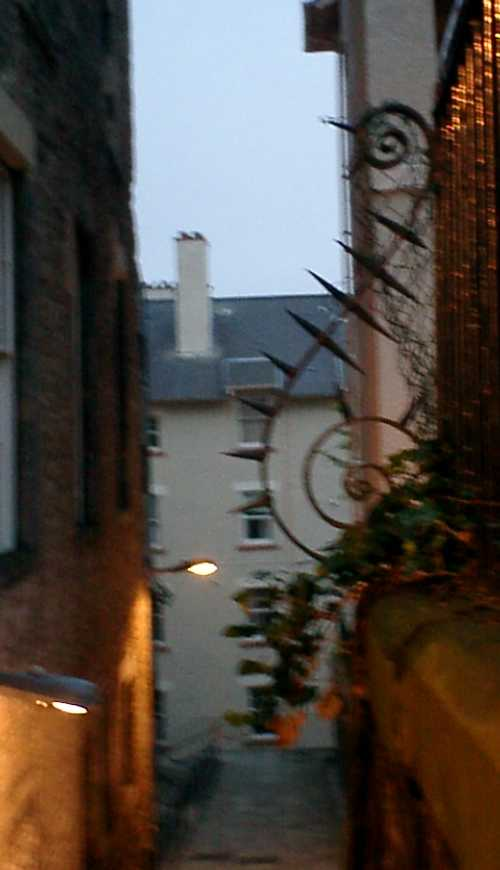
\includegraphics[width=1\hsize]{image200707/gurutitle.jpg}
\end{minipage}
\begin{minipage}{0.39\hsize}
 {\Huge #1
 }
\end{minipage}
\end{frame}
}

% 三択問題用
\newcounter{santakucounter}
\newcommand{\santaku}[5]{%
\addtocounter{santakucounter}{1}
\frame{\frametitle{問題\arabic{santakucounter}. #1}
%問題\arabic{santakucounter}. #1
\begin{minipage}[t]{0.8\hsize}
 \begin{itemize}
 \item
      \begin{minipage}{0.2\hsize}
      
\includegraphics[width=0.9\hsize]{image200703/janken-A.png}\end{minipage} 
       \begin{minipage}{0.6\hsize}
       A #2\end{minipage}\\
 \item
      \begin{minipage}{0.2\hsize}
      
\includegraphics[width=0.9\hsize]{image200703/janken-B.png}\end{minipage} 
       \begin{minipage}{0.6\hsize}
       B #3\end{minipage}\\
 \item
      \begin{minipage}{0.2\hsize}
      
\includegraphics[width=0.9\hsize]{image200703/janken-C.png}\end{minipage} 
       \begin{minipage}{0.6\hsize}
       C #4\end{minipage}\\
 \end{itemize}
\end{minipage}
}
\frame{\frametitle{問題\arabic{santakucounter}. #1}
%問題\arabic{santakucounter}. #1
\begin{minipage}[t]{0.8\hsize}
\begin{itemize}
 \item
      \begin{minipage}{0.2\hsize}
      
\includegraphics[width=0.9\hsize]{image200703/janken-A.png}\end{minipage} 
       \begin{minipage}{0.6\hsize}
       A #2\end{minipage}\\
 \item
      \begin{minipage}{0.2\hsize}
      
\includegraphics[width=0.9\hsize]{image200703/janken-B.png}\end{minipage} 
       \begin{minipage}{0.6\hsize}
       B #3\end{minipage}\\
 \item
      \begin{minipage}{0.2\hsize}
      
\includegraphics[width=0.9\hsize]{image200703/janken-C.png}\end{minipage} 
       \begin{minipage}{0.6\hsize}
       C #4\end{minipage}\\
\end{itemize}
\end{minipage}
\begin{minipage}[t]{0.15\hsize}
答えは:

\vspace{1cm}

  {\huge \hspace{1cm}#5}
  \hspace{-6cm}\includegraphics[width=4cm]{image200703/janken-#5.png}
 \end{minipage}}
}

\begin{document}

\frame{\titlepage{}}


\section{はじめに}

\begin{frame}{}
\begin{center}
本日は 日本 . ユーザ会 設立の発表をさせていただきます。
\end{center}
\end{frame}

\begin{frame}{}
\begin{center}
皆様、 日本 . ユーザ会 設立会に参加していただきありがとうございます。
\end{center}
\end{frame}

\begin{frame}{}
\begin{center}
日本 . ユーザ会 設立の趣旨
\end{center}
\begin{enumerate}
\item . の普及活動
\item . 開発者の育成
\item . ユーザの育成
\item . マニュアルの翻訳
\item など
\end{enumerate}

\end{frame}

\begin{frame}{}
\begin{center}
みなさん . つかっていますか?
\end{center}
\end{frame}

\begin{frame}{}
\begin{center}
ピリオドじゃないよ、ドットだよ。
\end{center}
\end{frame}

\begin{frame}{}
\begin{center}
dot / dot 言語
\end{center}
\end{frame}

\begin{frame}{}
\begin{center}
  グラフ構造などを作成するための言語。\\
DoxygenやGraphvizで使われている。
\end{center}
\end{frame}

\begin{frame}{}
\begin{center}
問題: このような関係図を描くには?\\
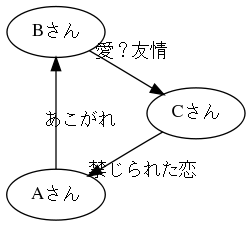
\includegraphics[width=0.5\hsize]{image200812/tl.png}
\end{center}
\end{frame}

\begin{frame}{}
\begin{center}
dot を使わない生活
\end{center}
\end{frame}

\begin{frame}{}
\begin{center}
パターン1\\
GIMP でちまちま描いて、画像ファイルに変換
\end{center}
\end{frame}

\begin{frame}{}
\begin{center}

\includegraphics[width=0.6\hsize]{image200812/pugya.png}
\end{center}
\end{frame}


\begin{frame}{}
\begin{center}
パターン2\\
ooimpress でシコシコ描いて、画像ファイルに変換
\end{center}
\end{frame}

\begin{frame}{}
\begin{center}

\includegraphics[width=0.5\hsize]{image200812/pu.png}
\end{center}
\end{frame}

\begin{frame}[containsverbatim]{}
\begin{center}
dot を使った場合
\begin{commandline}
$ cat /tmp/tl.dot
digraph "love_triangle" {
   size = "10.0, 10.0";
   "Aさん" -> "Bさん" [label = "あこがれ"];
   "Bさん" -> "Cさん" [label = "愛?友情"];
   "Cさん" -> "Aさん" [label = "禁じられた恋"];
}
\end{commandline}
\end{center}
\end{frame}


\begin{frame}[containsverbatim]{}
\begin{center}
dot で変換
\begin{commandline}
% dot -Kcirco -Tpng tl.dot -o tl.png 
\end{commandline}
\end{center}
\end{frame}

\begin{frame}{}
\begin{center}
まぁ、簡単なやつだと OOo や GMIP でもいいよね。
\end{center}
\end{frame}

\begin{frame}{}
\begin{center}
こんなファイルが作成される。
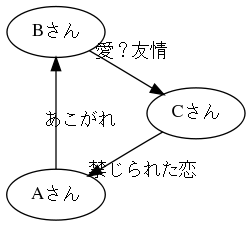
\includegraphics[width=0.5\hsize]{image200812/tl.png}
\end{center}
\end{frame}


%\begin{frame}{}
%%\begin{center}
%まったくそのとおり。
%\end{center}
%\end{frame}

\begin{frame}{}
\begin{center}
しかし、
\end{center}
\end{frame}

\begin{frame}{}
\begin{center}
Debian勉強会の Git コミット関係図を書きなさい。
ただし、最新コミットから60コミットおよび100コミット前までとする。
\end{center}
\end{frame}

\begin{frame}{}
\begin{center}
どうする?
\end{center}
\end{frame}

\begin{frame}{}
\begin{center}
GIMP や ooimpress ではけっこう死ねる\\
(かも。スクリプトでできる?知らん!)
\end{center}
\end{frame}

\begin{frame}[containsverbatim]{}
\begin{center}
dot を使った場合

\begin{commandline}
$ echo 'digraph git {' > /tmp/git.dot
$ git log --pretty='format:  %h -> { %p }'\
       "HEAD~100..HEAD~60" \ 
       | sed 's/[0-9a-f][0-9a-f]*/\"&\"/g' \ 
       >>  /tmp/git.dot
$ echo '}' >> /tmp/git.dot
\end{commandline}
\end{center}
\end{frame}

\begin{frame}[containsverbatim]{}
\begin{center}
ファイルの中身

\begin{commandline}
$ cat /tmp/git.dot
digraph git {
  "60a5b09" -> { "ceed540" }
  "ceed540" -> { "2c4d400" }
  "2c4d400" -> { "145e2b5" }
  "145e2b5" -> { "e95203a" }
  "e95203a" -> { "3c72eb6" }
  "3c72eb6" -> { "1742d57" }
  "1742d57" -> { "762a999" }
  "762a999" -> { "efbea15" }
.....
\end{commandline}
\end{center}
\end{frame}

\begin{frame}[containsverbatim]{}
\begin{center}
実行する
\begin{commandline}
$ dot -Kneato -Tpng /tmp/git.dot -o /tmp/git.png
\end{commandline}
\end{center}
\end{frame}

\begin{frame}{}
こんな感じになります。
\begin{center}
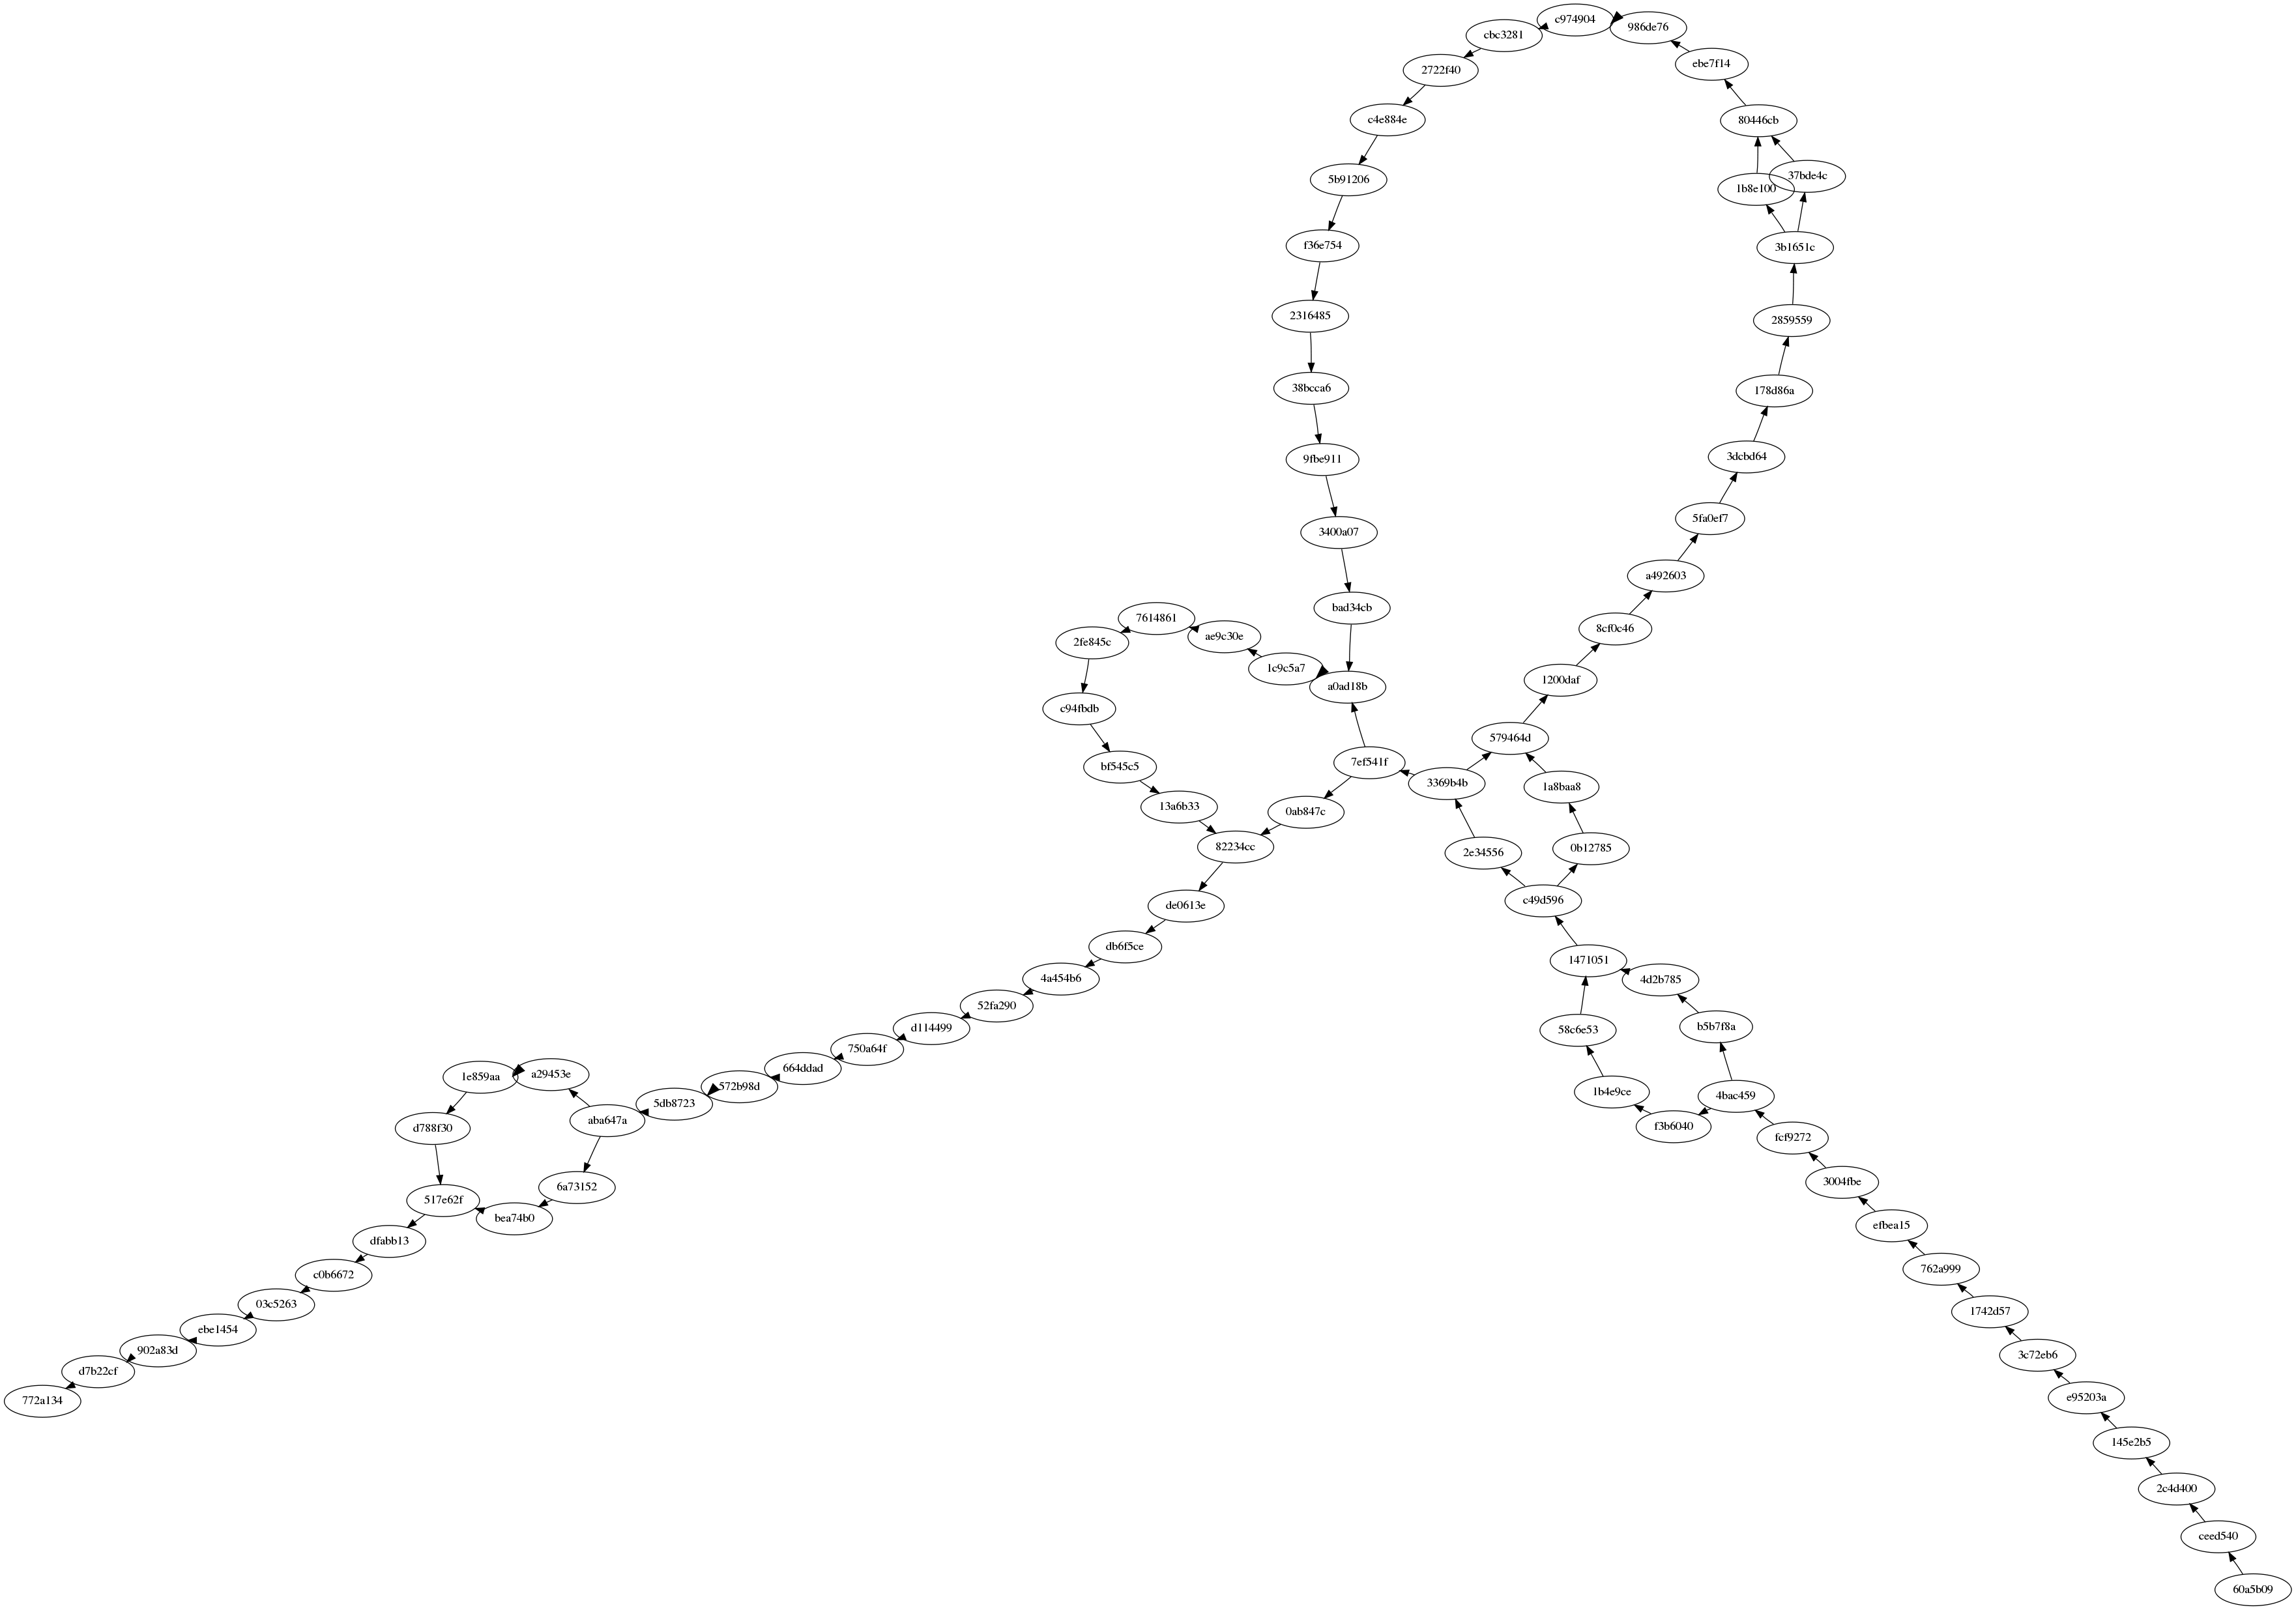
\includegraphics[width=1.0\hsize]{image200812/git.png}
\end{center}
\end{frame}

\begin{frame}{}
先日発表された「あたし状態遷移図」も dot (graphviz)!
\end{frame}

\begin{frame}{}

\begin{center}
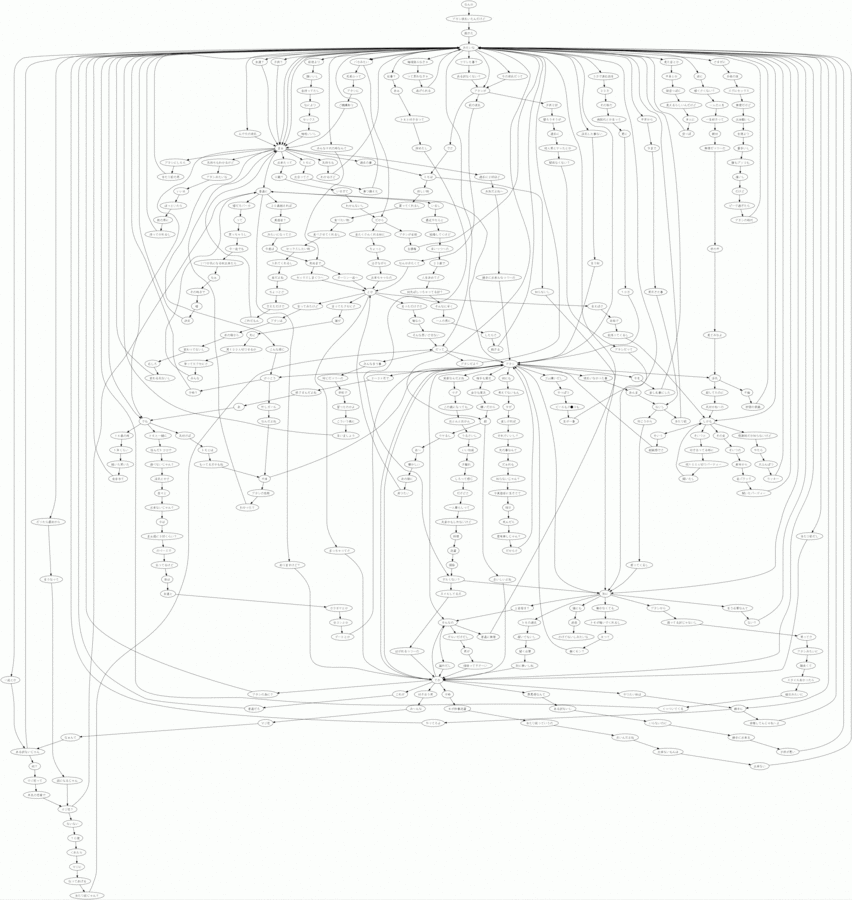
\includegraphics[width=1.0\hsize]{image200812/watashi-graph.png}
\end{center}
\footnote{http://neo.g.hatena.ne.jp/debedebe/20081218/1229533744}
\end{frame}

\begin{frame}{}
\begin{itemize}
 \item 様々な画像ファイルフォーマットへの対応。\\
    png,jpeg,gif,tif etc...
 \item 描画アルゴリズムも5種類ある。\\
    circo, dot, fdp, neato, twopi

\end{itemize}
\end{frame}

\begin{frame}{}
%dot(有向グラフ)
\begin{center}
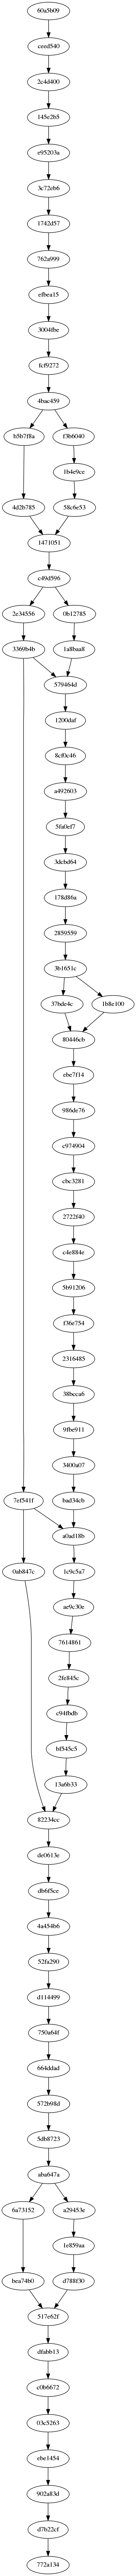
\includegraphics[width=0.2\hsize]{image200812/git-dot.png}
\end{center}
\end{frame}

\begin{frame}{}
%twopi(放射状レイアウト)
\begin{center}
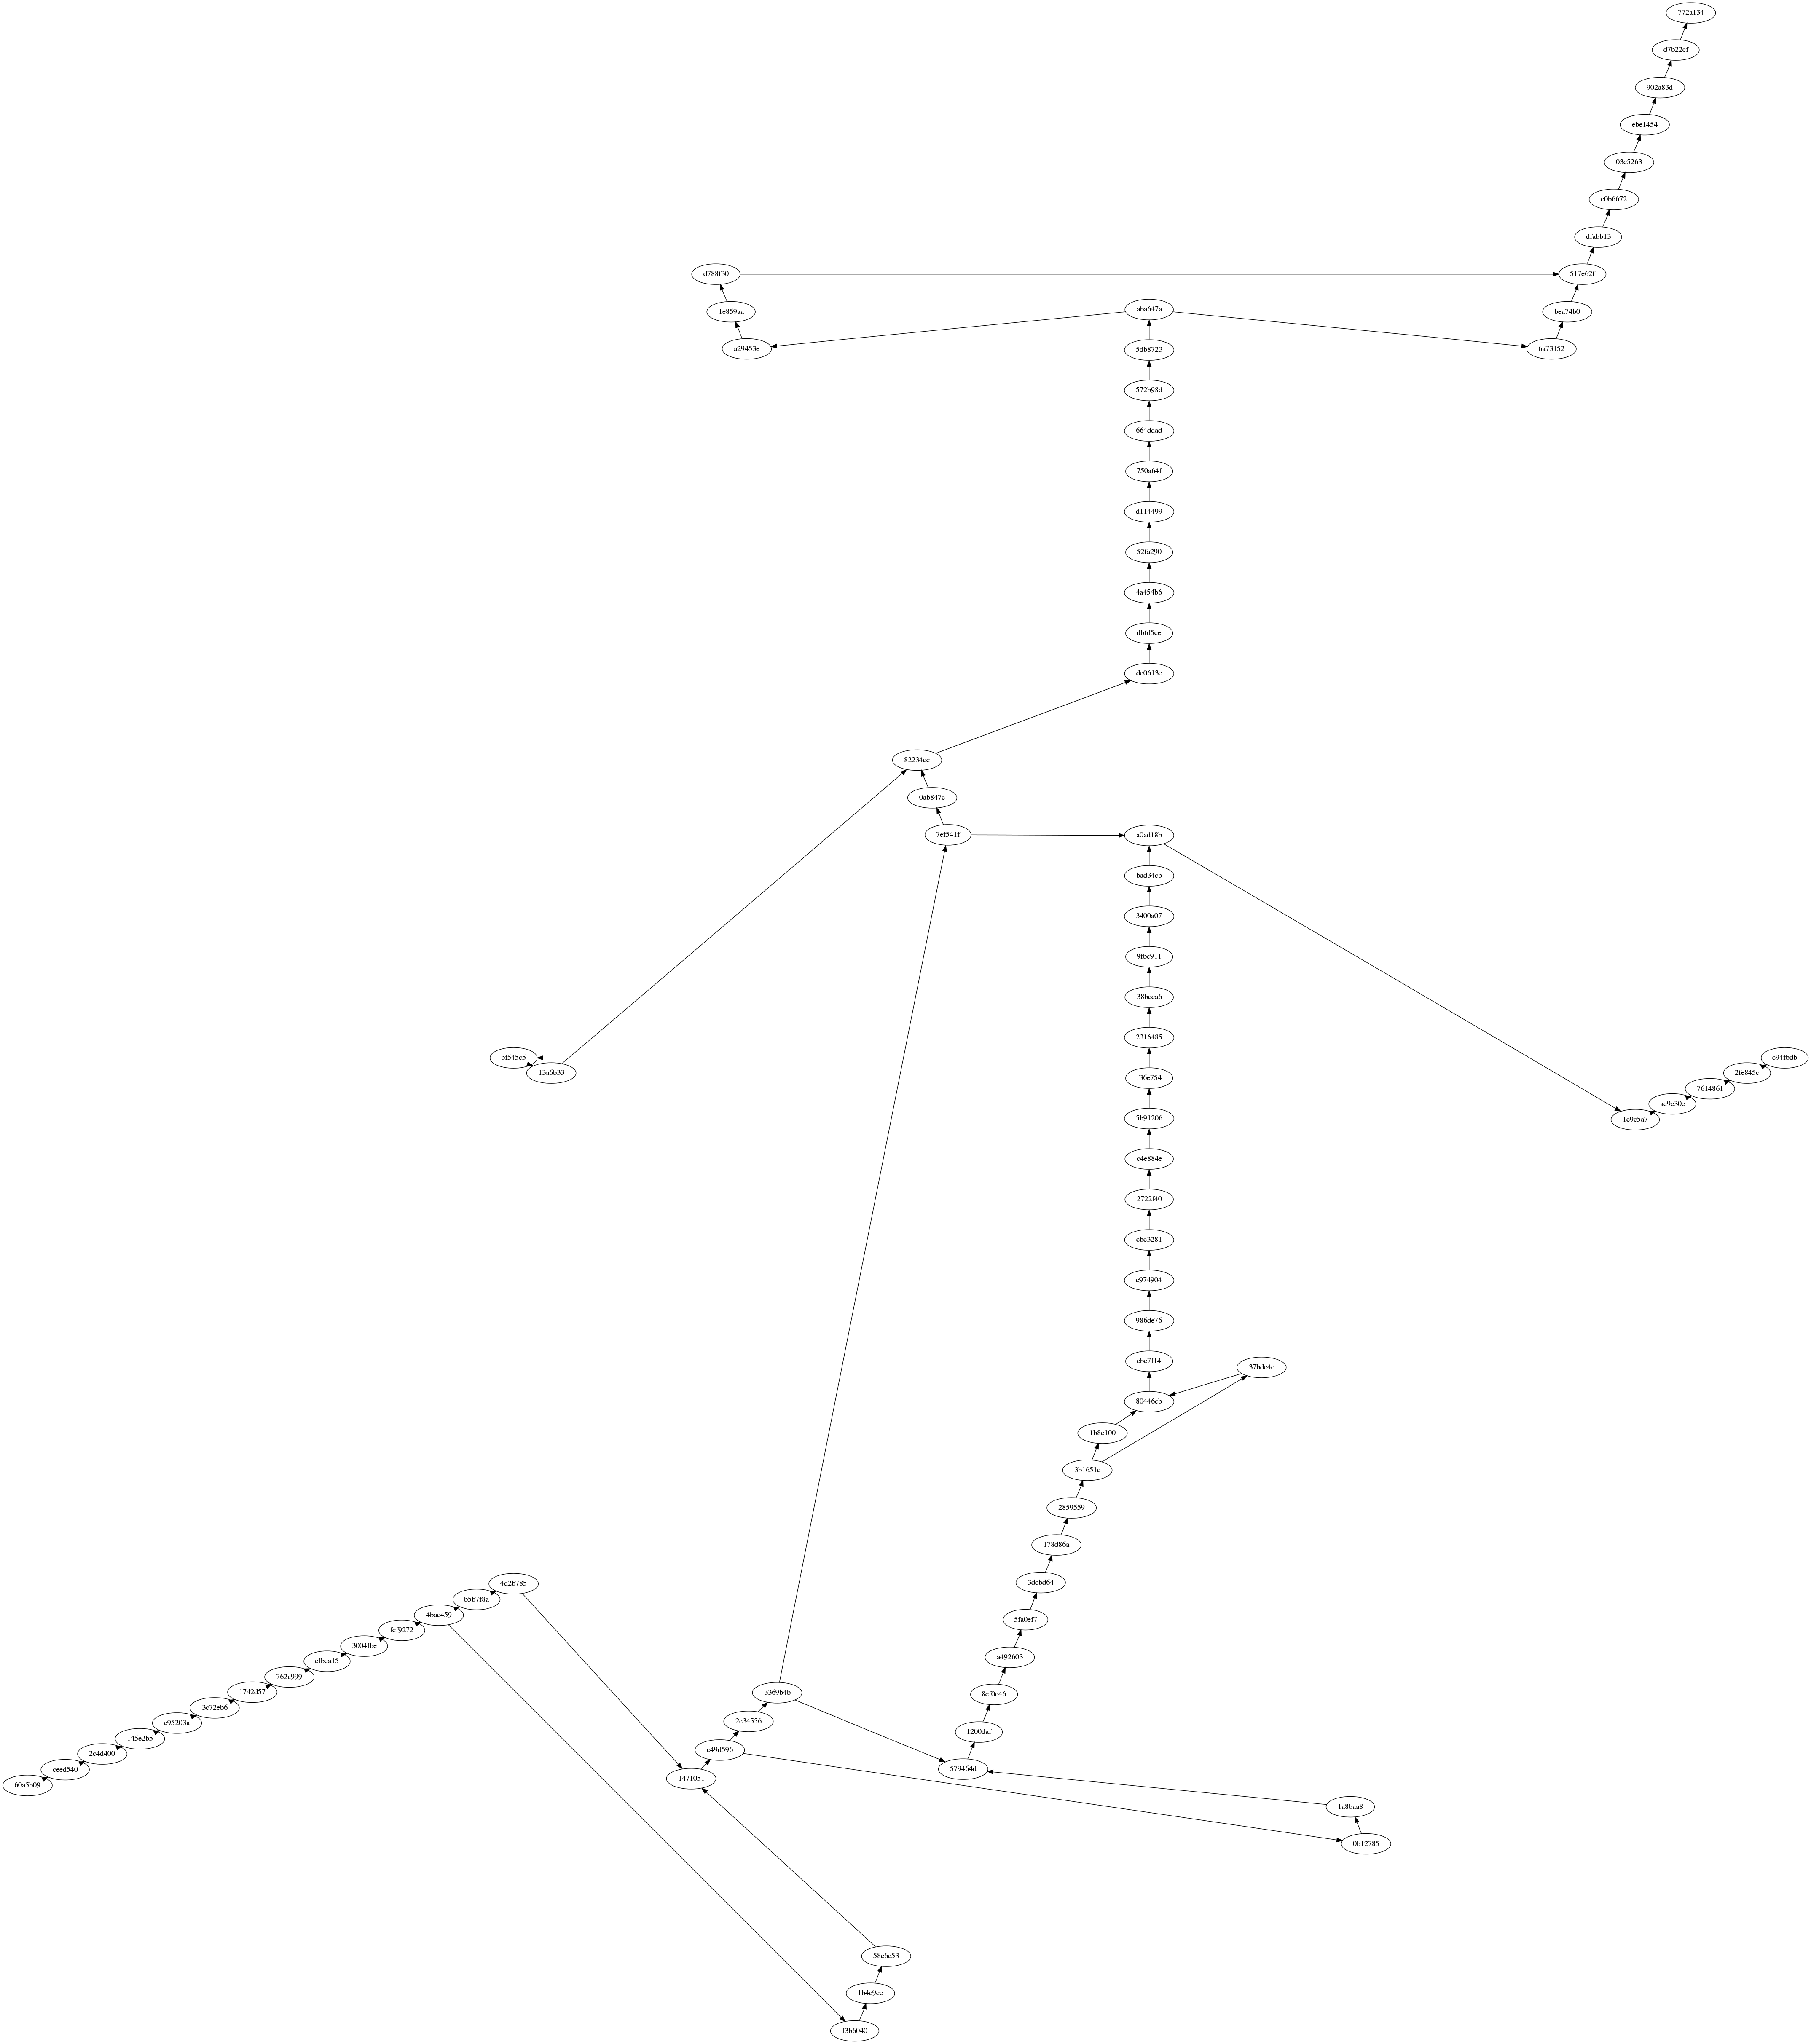
\includegraphics[width=0.8\hsize]{image200812/git-twopi.png}
\end{center}
\end{frame}

\begin{frame}{}
%fdp(無向グラフ)
\begin{center}
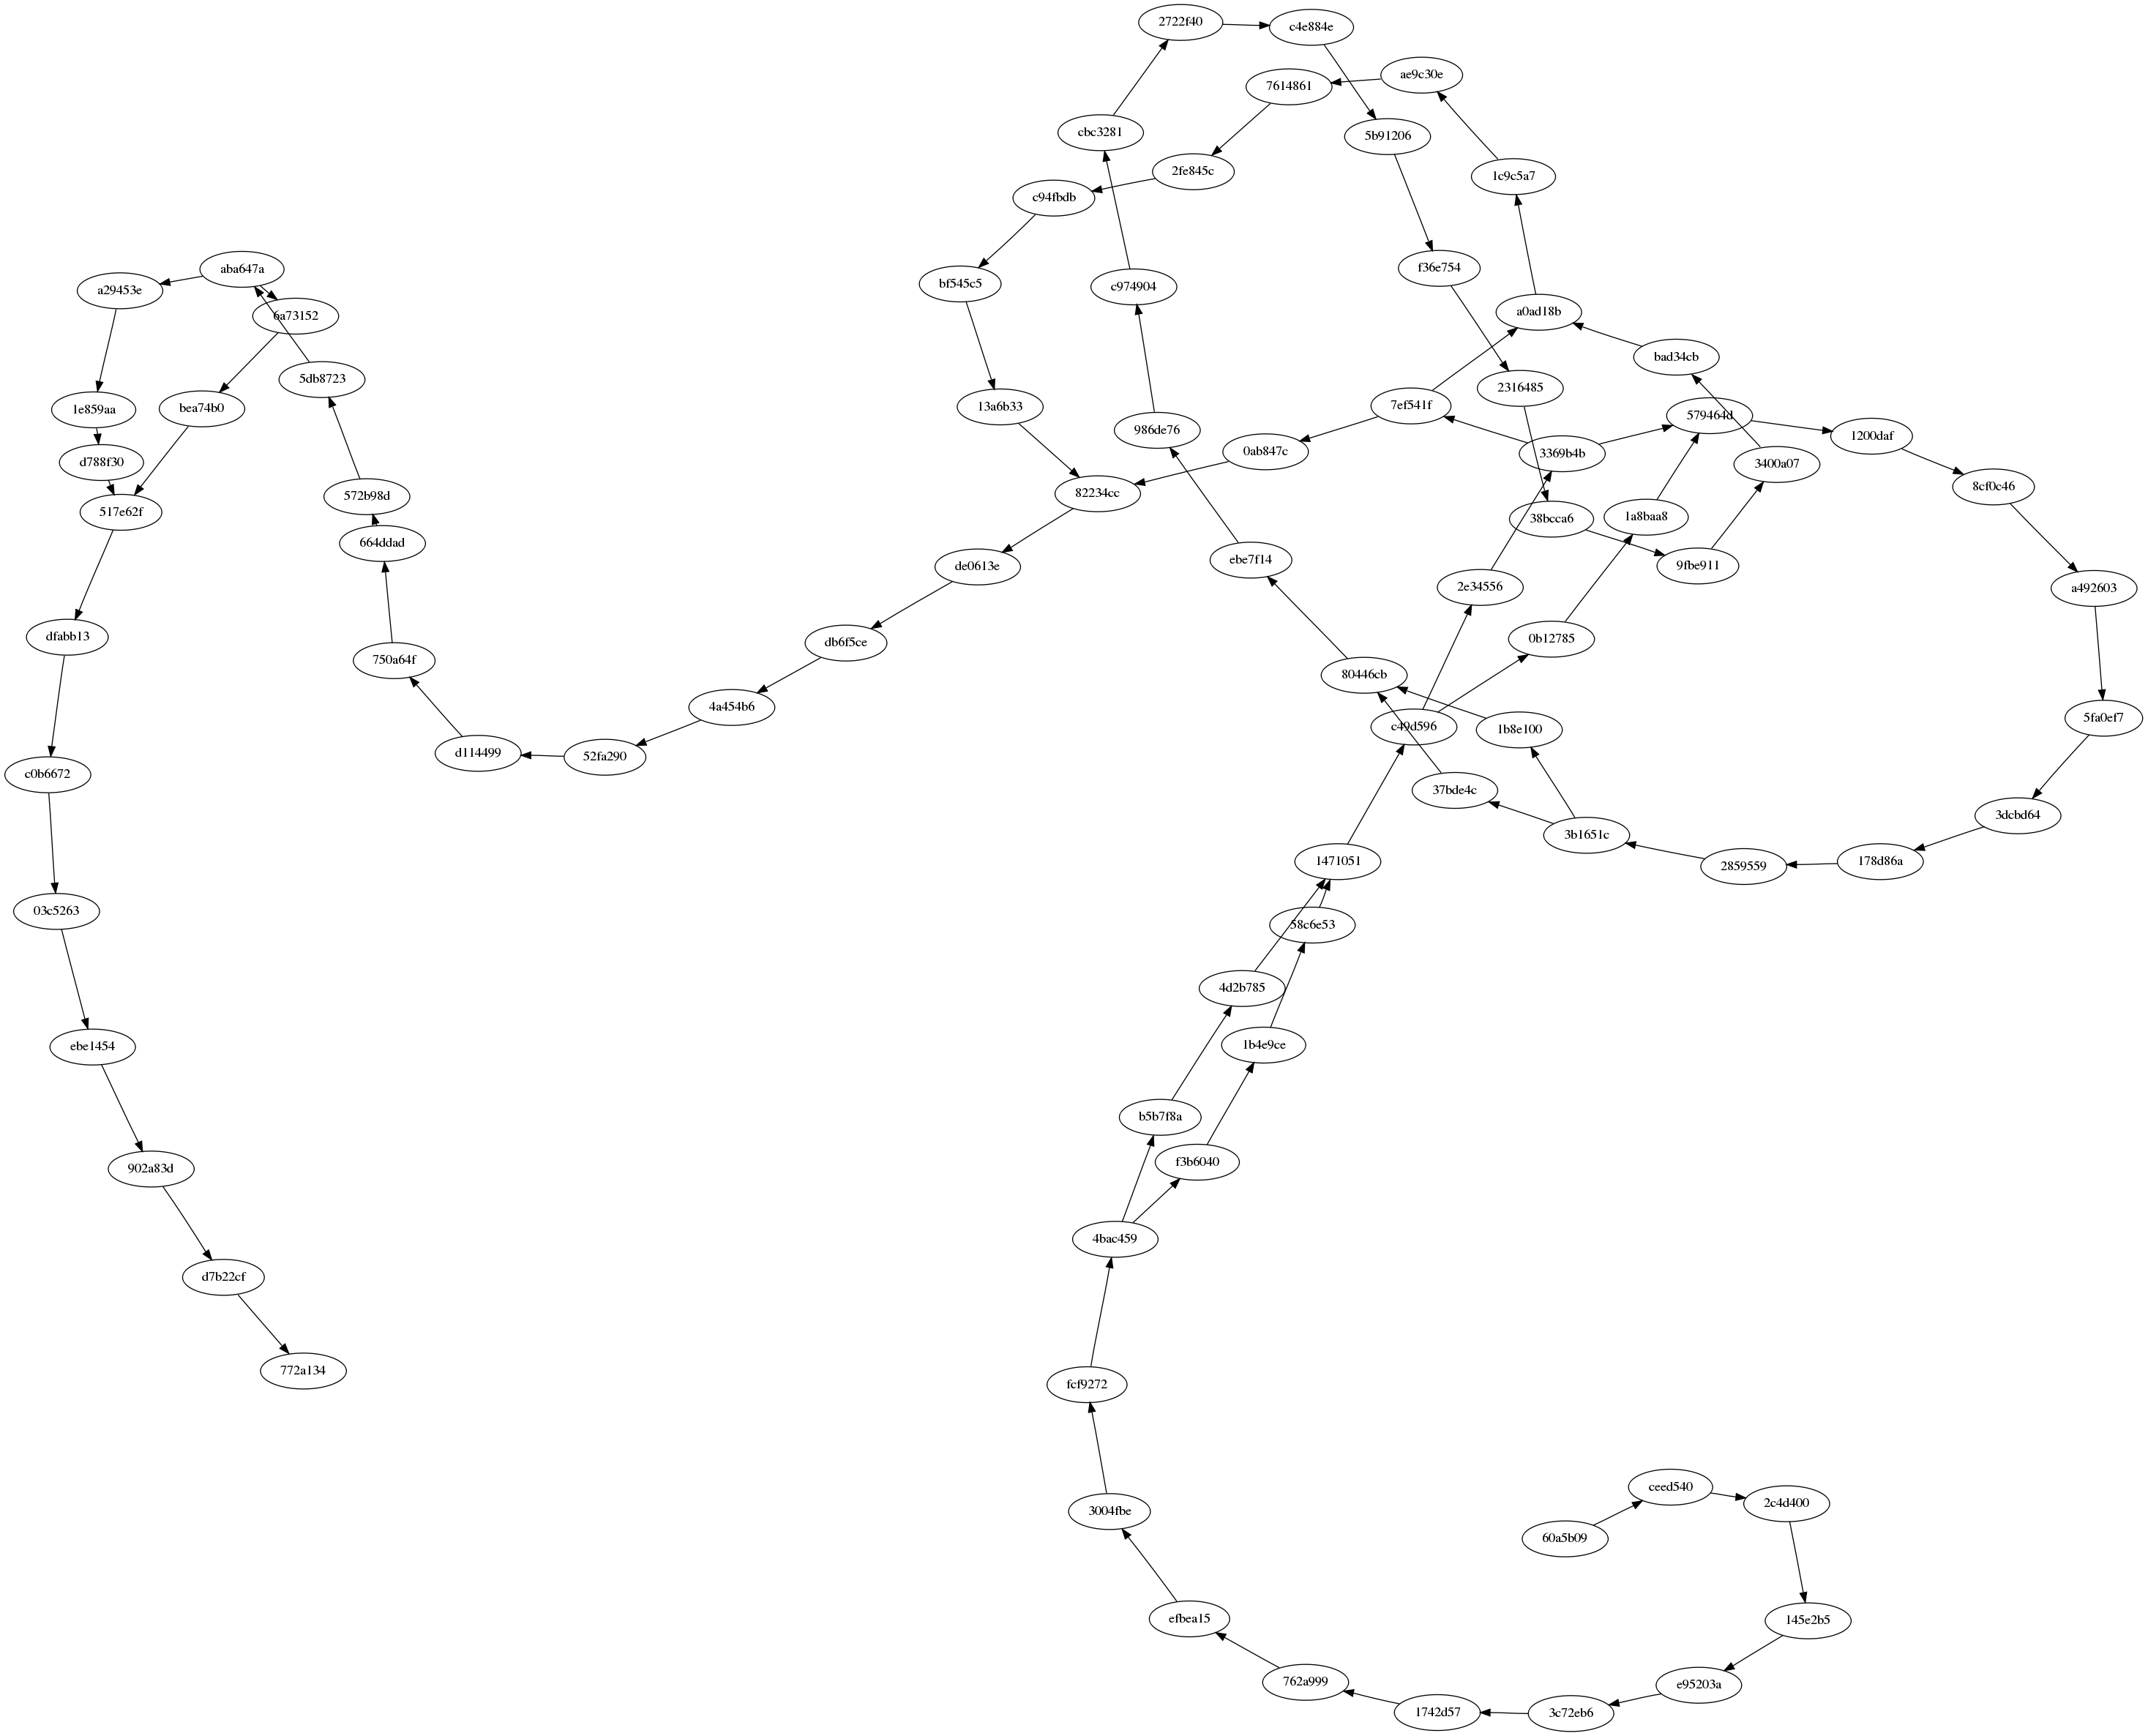
\includegraphics[width=0.8\hsize]{image200812/git-fdp.png}
\end{center}
\end{frame}

\begin{frame}{}
\begin{itemize}
 \item テキストなので差分が管理できるという利点\\
     編集も容易
 \item スクリプトでゴリゴリ書けたり。
\end{itemize}
\end{frame}

\begin{frame}{}
\begin{center}
Debian 勉強会でも約2名ほど使っています。\\
(上川さんと岩松だけ?)
\end{center}
\end{frame}

\begin{frame}{}
\begin{center}
Debian勉強会では今後は dot を使うことを推奨します。(たぶん。)
\end{center}
\end{frame}

\begin{frame}{}
\begin{center}
なので、Debian勉強会参加者は強制参加です。
\end{center}
\end{frame}

\begin{frame}{}
\begin{center}
以上で、日本 . ユーザ会 設立 の言葉と変えさせていただきます。
\end{center}
\end{frame}

\begin{frame}{}
\begin{center}
ありがとうございました。
\end{center}
\end{frame}

\begin{frame}{}
\begin{center}
日本 . ユーザ会 解散のお知らせ
\end{center}
\end{frame}

\begin{frame}{}
\begin{center}
言いたいことは言ったので、\\
日本 . ユーザ会 は解散します。
これまでありがとうございました。
\end{center}
\end{frame}


\end{document}

;;; Local Variables: ***
;;; outline-regexp: "\\([ 	]*\\\\\\(documentstyle\\|documentclass\\|emtext\\|section\\|begin{frame}\\)\\*?[ 	]*[[{]\\|[]+\\)" ***
;;; End: ***
